%------------------------------------------------------------------------
\chapter{Godlowskian Transformation}\label{God}
%------------------------------------------------------------------------
The derivation of the basic formula is given considering the
distribution of galaxies within the LSC \& its PA in galactic
system. Let us consider a equatorial coordinate system, hereafter
referred to as the E system. An observer is situated at the origin
of the E system which is at the center of our galaxy. The X-Y
plane represents the plane of the E system (i.e, the plane of the
Milky way) and the coordinates $\alpha$ and $\delta$ represent the
equatorial longitude and latitude, respectively. The X-axis,
called EX is directed towards the center of the equatorial plane
($\alpha$ = 0, $\delta$ = 0). The Y and Z-axis known as EY and EZ
are directed towards the point $\alpha$ = $\pi$/2, $\delta$ = 0
and north equatorial pole ($\alpha$ = $\pi$/2, $\delta$ =
$\pi$/2), respectively.
\\
\\
Let us consider another coordinate system. The origin of the this
system is at the galaxy center. In this system, U and V-axes are
perpendicular to each other and tangent to the celestial sphere.
The U-axis is parallel to the equatorial latitude. The W-axis is
perpendicular to both U and V-axes and is the extension of the
connecting line between the centers of the cluster to the center
of galaxy. This axis points out of the sphere. These can be seen
in Fig. A1. Fig. A2 shows the detailed view of the galaxy
showing the vectors described above. The angle $q$ is an angle
between the U-axis and the projection of galaxy major axis $a$ on
the celestial sphere. The minor axis is denoted by $b$. The angle
$q$ is related to the equatorial position angle $p$, measured in
the equatorial coordinate system is given by the expression: $q$ =
$p$$-$$\pi$/2 and is measured from $-$$\pi$/2 to $+$$\pi$/2.
\\\\
\begin{figure} \vspace{0.0cm}
      \centering
      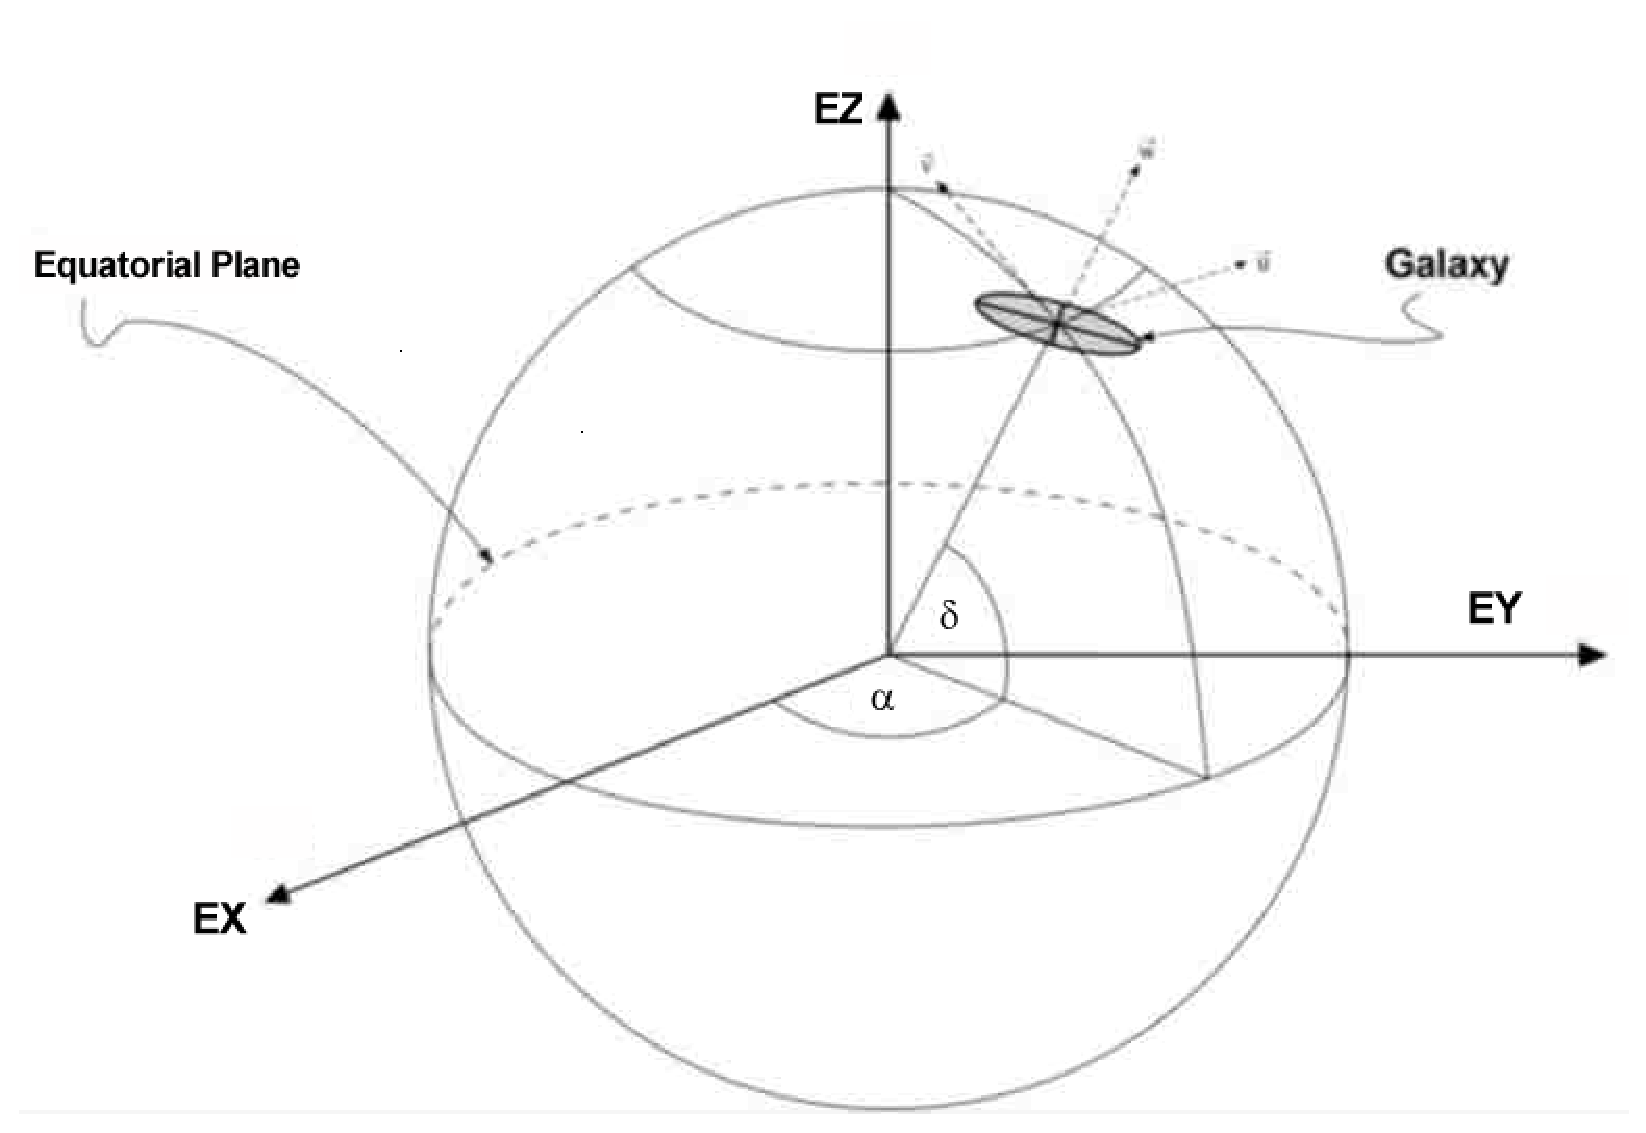
\includegraphics[height=10cm]{Godlowski1}
      \caption[]{The coordinate system used for the derivation of the polar and
azimuthal angle of the galaxy rotation axes. Here $\alpha$ and
$\delta$ represent right ascension and declination of the galaxy.
[source: Aryal 2002] }
\end{figure}
\begin{figure} \vspace{0.0cm}
      \centering
      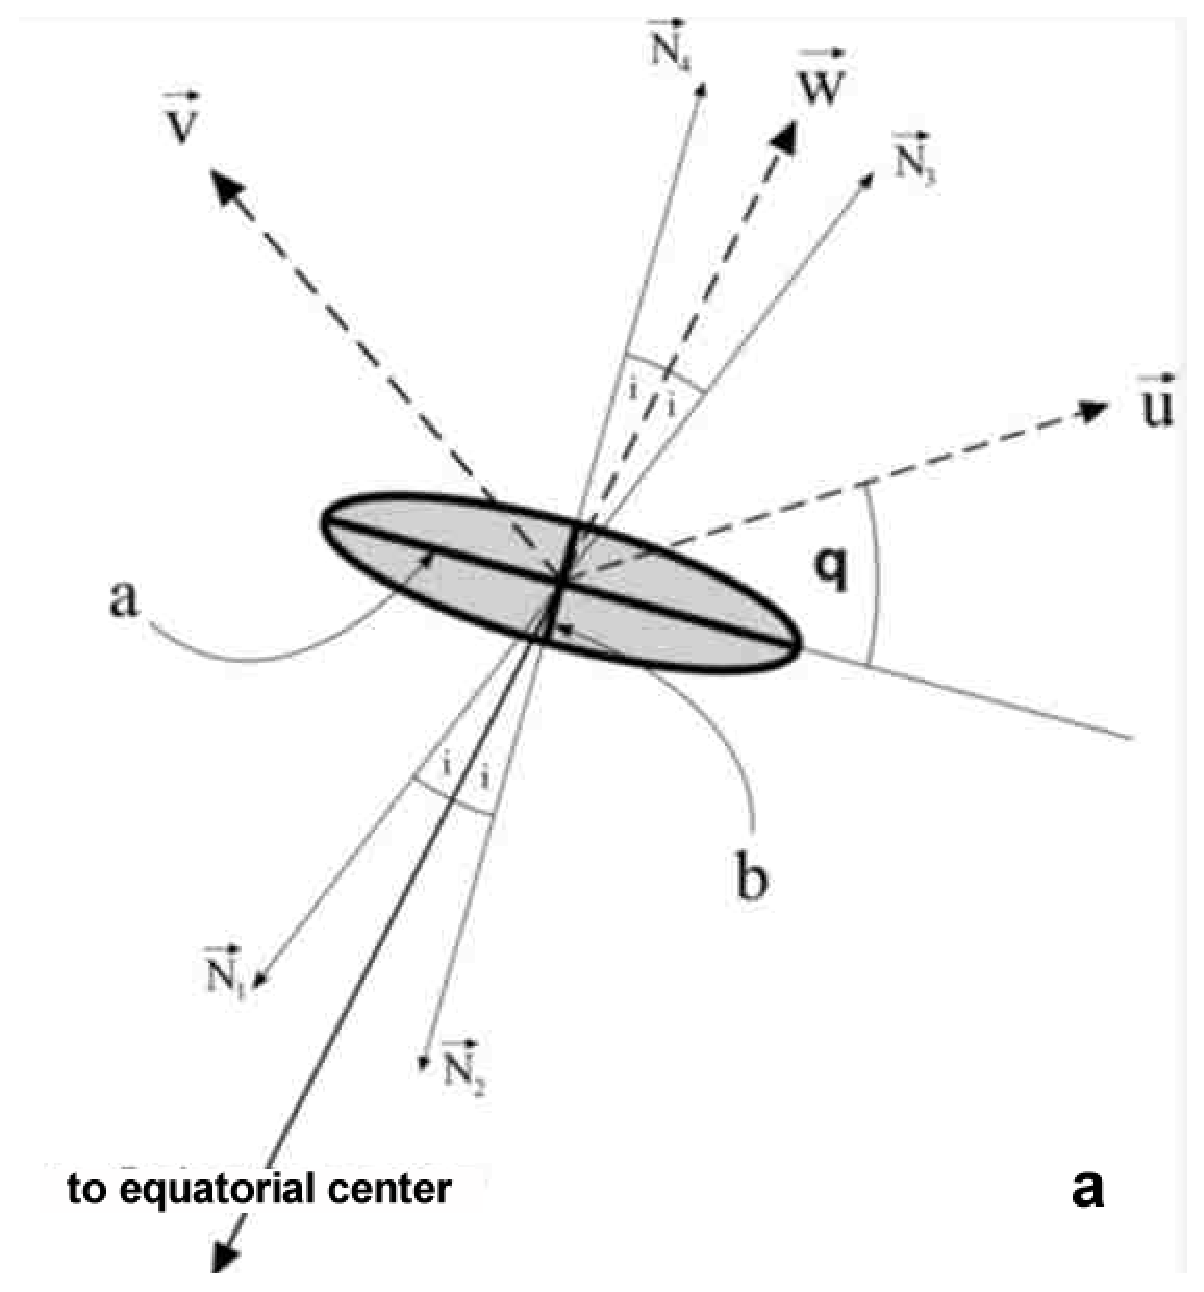
\includegraphics[height=7.7cm]{Godlowski2}
      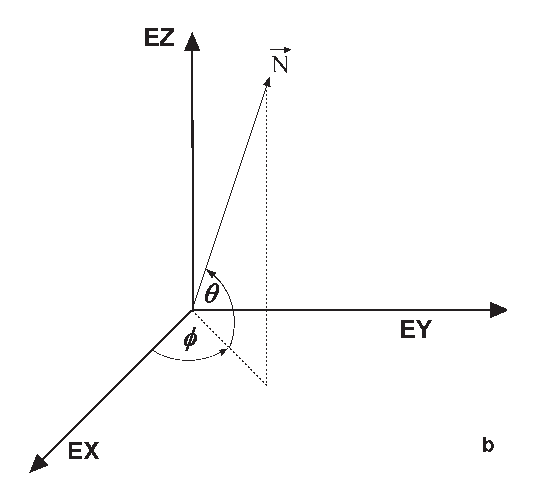
\includegraphics[height=7.7cm]{Godlowski3}
      \caption[]{(a) Detailed view on a galaxy: $a$ and $b$ are the major
      and the minor axes, $q$ = $p$ -- $\pi$/2, N$_1$ and N$_2$ corresponds to the
      two possible rotation axes. (b) Definition of the two angles $\theta$ and $\phi$
      which contain the orientation of the spin vector $N$ with respect
      to the equatorial coordinate system. [source: Aryal 2002]}
\end{figure}
\\
\\
Let us extend the normal to the galaxy plane passing through the
origin of equatorial system. For an inclination angle, $i$, there
will be two possible normals N$_1$ and N$_2$, and hence two
possible positions of the galaxy rotation axis. The angular
momentum vector is situated along one of these two normals.  Let
us consider N$_1$ and N$_2$ as the galaxy angular momentum
vectors. It is seen from the Fig. A2.a that there are other two
spin vectors N$_3$ and N$_4$ oriented just opposite to N$_1$ and
N$_2$. N$_1$ and N$_3$ can be identified as one rotation axis
whereas N$_2$ and N$_4$ as second rotation axis. So the ambiguity
of four solutions for the spin vectors can be reduced to an
ambiguity of two solutions. Therefore just N$_1$ and N$_2$ are
used for the statistical investigation.
\\
\\
The vectors N$_1$ and N$_2$ in the E system are
\begin{equation}\label{N}
\begin{array}{l}
$N$_1$$ = - W\cos i + \sin i (V \cos q + U \sin q)\\
\\
$N$_2$$ = - W\cos i - \sin i (V \cos q + U \sin q)\\
\end{array}
\end{equation}
%----------------------------------------------------------------------------------
Where cos$i$ is given by Holmberg's equation with the flatness
factor q* and is
%----------------------------------------------------------------------------------
\begin{equation}
\begin{array}{l}
\cos^2 i = \frac{[(b/a)^2 - (q*)^2]}{1 - (q*)^2}
\end{array}
\end{equation}
%----------------------------------------------------------------------------------
and ($V\cos q\, +\, U\sin q$) is the projection of the normals to the U-V
plane. Now we apply the method of coordinate translation here. The
galaxy related reference frame is translated to the center of the
E system. This translation allows us to express the coordinates U,
V and W in the E system. In the E system, these coordinates are
the functions of right ascension ($\alpha$) and declination
($\delta$) only and they can be written as follows:
%-------------------------------------------------------------------------------
\begin{equation}\label{UVW}
\begin{array}{l}
U = (-\sin \alpha, \ cos \alpha, 0)\\
\\
V = (-\sin \delta\cos \alpha, \cos \delta\sin \alpha, \cos \delta)\\
\\
W = (\cos \delta\cos \alpha, \cos \delta\sin \alpha, \sin \delta)\\
\\
\end{array}
\end{equation}
%--------------------------------------------------------------------------------
here, $-$sin$\alpha$, cos$\alpha$ and 0 are the functions of the
vector U along X, Y and Z axes, respectively. Similarly,
$-$sin$\delta$cos$\alpha$, $-$sin$\delta$sin$\alpha$, cos$\delta$
and cos$\delta$cos$\alpha$, cos$\delta$sin$\alpha$, sin$\delta$
are the functions of the vectors V and W along X, Y and Z
directions, respectively.
\\
\\
Substituting the values of U, V and W from equation \eqref{UVW} in
\eqref{N} we get,
%------------------------------------------------------------------------------------
\begin{equation}\label{N_12}
\begin{array}{l}
$N$_{ix}$$ = - \cos i\cos \delta\cos \alpha + \sin i(\mp \cos q \sin \delta \cos \alpha \mp \sin q\sin \alpha); \\
\\
$N$_{iy}$$ = - \cos i\cos \delta\sin \alpha + \sin i(\mp \cos q \sin \delta \sin \alpha \pm \sin q\cos \alpha); \\
\\
$N$_{iz}$$ = - \cos i\cos \delta \pm \sin i\cos q\cos \delta ; \\
\end{array}
\end{equation}
%-------------------------------------------------------------------------------------

where the upper and lower signs are for $i$ =1 and 2,
respectively.
\\
\\
Now we introduce two angles: polar ($\theta$) and azimuthal angle
($\phi$) of galaxy rotation axis. The polar angle ($\theta$), is
the angle between the N$_i$ vector and the galactic plane. The
angle between the X-axis and the projection of the N$_i$ vector on
the galactic plane is termed as the azimuthal angle ($\phi$). It
should be noted that the reversal of the vectors N$_1$ and N$_2$
transforms the $\theta$ and $\phi$ values into $-$$\theta$ and
$\phi$ + $\pi$., respectively.
\\
\\
From Fig. A2 b, we can write,
\begin{equation}\label{theta_phi}
\begin{array}{l}
$N$_{ix}$$ =  \cos \theta\cos \phi; \\
\\
$N$_{iy}$$ =  \cos \theta\sin \phi;  \\
\\
$N$_{iz}$$ =  \sin \theta. \\
\end{array}
\end{equation}\\
%--------------------------------------------------------------------------------
Comparing the equations \eqref{theta_phi} and \eqref{N_12} gives,
%-------------------------------------------------------------------------------
\begin{equation}\label{theta_phi_delat1}
\begin{array}{l}
\sin \theta = -\cos i\sin \delta \pm \sin i\cos q\cos \delta;\\
\\
\sin \phi = \frac{- \cos i\cos \delta\sin \alpha + \sin i(\mp \cos q \sin \delta\sin \alpha \pm \sin q\cos \alpha)}{\cos \theta};\\
\\
\cos \phi = \frac{- \cos i\cos b\cos \alpha + \sin i(\mp \cos q \sin \delta\cos \alpha \mp \sin q\sin \alpha)}{\cos \theta}.\\
\end{array}
\end{equation}\\
%---------------------------------------------------------------------------------------
Substituting q = $p$ $-$ $\pi$/2 in equation \eqref{theta_phi_delat1},
%--------------------------------------------------------------------------------------
\begin{equation}\label{theta_phi_delta2}
\begin{array}{l}
\sin \theta = -\cos i\sin \delta \pm \sin i\sin p\cos \delta;\\
\\
\sin \phi = \frac{- \cos i\cos \delta\sin \alpha + \sin i(\mp \sin p \sin \delta\sin \alpha \mp \cos p\cos \alpha)}{\cos \theta};\\
\\
\cos \phi = \frac{- \cos i\cos \delta\cos \alpha + \sin i(\mp \sin p \sin \delta\cos \alpha \pm \cos p\sin \alpha)}{\cos \theta}.\\
\end{array}
\end{equation}
\\
%----------------------------------------------------------------------------------------
Using equation \eqref{theta_phi_delta2}, the spin vector orientation of a galaxy can
be derived. These equations \eqref{theta_phi_delat1} and \eqref{theta_phi_delta2} derived above are
called `Godlowski-Transformation' or `Godlowskian Model'. In the
equation \eqref{theta_phi_delta2} the position parameters are equatorial system
parameters. In addition to this, we use position parameters for
galactic (l, b) and Supergalactic (L,B) coordinate system, as
follows.
\\
\begin{equation}\label{lb}
\begin{array}{l}
\sin \theta = -\cos i\sin b \pm \sin i\sin p\cos b;\\
\\
\sin \phi = \frac{- \cos i\cos b\sin l + \sin i(\mp \sin p \sin b\sin l\mp \cos p\cos l)}{\cos \theta};\\
\\
\cos \phi = \frac{- \cos i\cos b\cos l + \sin i(\mp \sin p \sin b\cos l \pm \cos p\sin l)}{\cos \theta}.\\
\end{array}
\end{equation}\\
\\
\begin{equation}\label{LB}
\begin{array}{l}
\sin \theta = -\cos i\sin B \pm \sin i\sin P\cos B;\\
\\
\sin \phi = \frac{- \cos i\cos B\sin L + \sin i(\mp \sin P \sin B\sin L\mp \cos P\cos L)}{\cos \theta};\\
\\
\cos \phi = \frac{- \cos i\cos B\cos L + \sin i(\mp \sin P \sin B\cos L \pm \cos P\sin L)}{\cos \theta}.\\
\end{array}
\end{equation}
\\
Expressions \eqref{theta_phi_delta2}, \eqref{lb} and \eqref{LB} give two solutions for both
$\theta$ and $\phi$ for a given value of $i$. Hence 4 solutions
are obtained for the angular momentum vector of the galaxy.
However, for a large sample of galaxies it is hardly possible to
determine - for each galaxy - which one is the physical correct
one. We count each of these possibilities independently for
statistical analysis.
\\
\\
The expressions \eqref{theta_phi_delta2}, \eqref{lb} and \eqref{LB} give single solution for both
$\theta$ and $\phi$ when a galaxy is seen exactly face-on ($i$ =
0$^{\circ}$). When seen edge-on ($i$ = 90$^{\circ}$), the two
solutions for both and differ just in sign. In the case of
$\theta$, both solutions converge when approaching the equatorial
pole or for galaxies with equatorial PA = 0$^{\circ}$. In the case
of $\phi$, both solutions just differ in sign for $\alpha$ =
0$^{\circ}$. More interestingly, the characteristics of the
solutions for and are also strongly influenced by the used
coordinate system. This was already noted by Flin \& Godlowski
(1986). These authors suggested an analytical method to remove
these selection effects due to positions.
